\begin{frame}{Atraminių vektorių klasifikatorius}
    \begin{columns}
        \begin{column}{0.5\textwidth}
            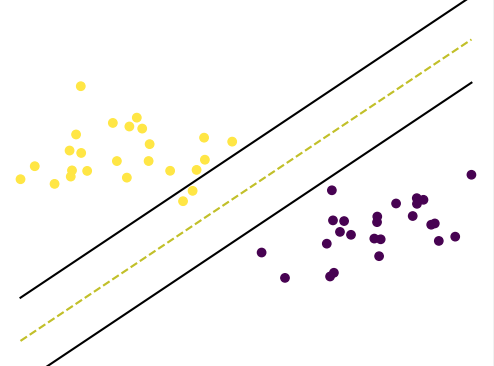
\includegraphics[scale=0.45]{img/svm.png}
        \end{column}
    
        \begin{column}{0.4\textwidth}
        Mažiausių kvadratų atraminių vektorių klasifikatoriaus (LSSVM) forma \cite{LSSVM}:
            \begin{equation}
                \begin{bmatrix}
                    0 & \vec{1}_N^T \\
                    \vec{1}_N & \Omega + \gamma^{-1} I_N
                \end{bmatrix} \cdot 
                \begin{bmatrix}
                    d \\
                    \vec{\theta}
                \end{bmatrix} = 
                \begin{bmatrix}
                    0 \\
                    \vec{y}    
                \end{bmatrix} \nonumber
            \end{equation}
            
            $\vec{1}_N = {\underbrace{[1;\ldots; 1]}_{N}}^T$, $\Omega = X^T X$ - tiesinė branduolio matrica, $\gamma$ - reguliavimo parametras, $d$ - poslinkio reikšmė, $\vec{\theta}$ - Lagranžo daugikliai , $\vec{y}$ - duomenų aibės klasių reikšmės.
        \end{column}
    \end{columns}
\end{frame}